\documentclass[tikz, border=3.14mm]{standalone}
\usepackage{pgfplots}
\pgfplotsset{compat=1.18}
\usepgfplotslibrary{groupplots}

\begin{document}
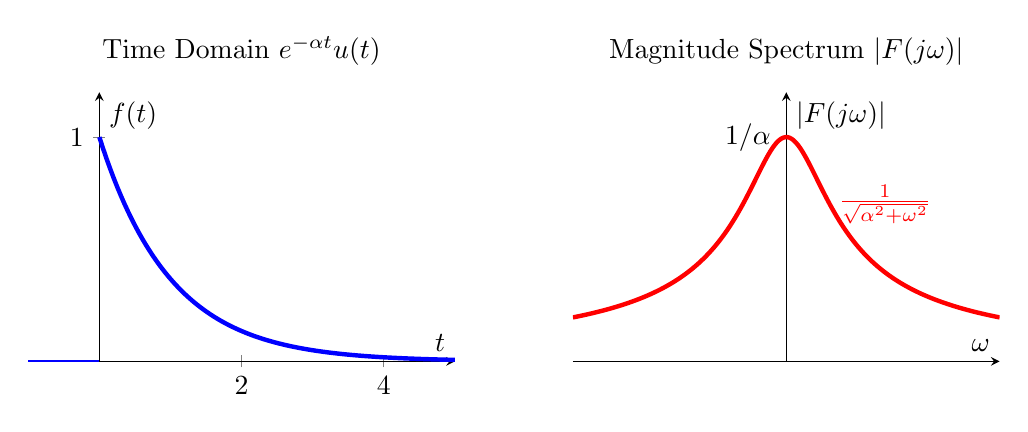
\begin{tikzpicture}
    \begin{groupplot}[
        group style={group size=2 by 1, horizontal sep=1.5cm},
        axis lines = middle,
        width = 7cm, height = 5cm,
        grid=none,
        xlabel = {$t$},
        ylabel = {$f(t)$}
    ]
        % Time Domain Exponential Decay
        \nextgroupplot[
            title = {Time Domain $e^{-\alpha t}u(t)$},
            xmin = -1, xmax = 5,
            ymin = 0, ymax = 1.2,
            ytick = {1},
            yticklabels = {$1$}
        ]
        \addplot[ultra thick, blue, domain=0:5, samples=100] {exp(-x)};
        \draw[blue, thick] (-1,0) -- (0,0);

        % Frequency Domain Magnitude
        \nextgroupplot[
            title = {Magnitude Spectrum $|F(j\omega)|$},
            xlabel = {$\omega$},
            ylabel = {$|F(j\omega)|$},
            xmin = -5, xmax = 5,
            ymin = 0, ymax = 1.2,
            ytick = {1},
            yticklabels = {$1/\alpha$},
            xtick = \empty
        ]
        \addplot[ultra thick, red, domain=-5:5, samples=200] {1/sqrt(1 + x^2)};
        \node[anchor=west, red] at (axis cs:1, 0.7) {$\frac{1}{\sqrt{\alpha^2 + \omega^2}}$};

    \end{groupplot}
\end{tikzpicture}
\end{document}
